\documentclass[tikz,border=4pt]{standalone}
% Shared style for every figure and for the deck: one accent, one
% highlight, thin lines, rounded nodes, nothing decorative.
\usepackage[T1]{fontenc}
\usepackage{lmodern}
\renewcommand{\familydefault}{\sfdefault}
\usepackage{tikz}
\usetikzlibrary{arrows.meta,positioning,calc,shapes.misc,fit,backgrounds,decorations.pathreplacing}
\definecolor{ink}{RGB}{40,40,40}
\definecolor{soft}{RGB}{150,150,150}
\definecolor{faint}{RGB}{225,225,225}
\definecolor{accent}{RGB}{0,95,115}
\definecolor{accentlight}{RGB}{214,232,236}
\definecolor{warn}{RGB}{196,84,40}
\definecolor{warnlight}{RGB}{247,226,216}
\tikzset{
  every picture/.style={color=ink, line width=0.5pt, font=\small},
  node distance=12mm and 18mm,
  box/.style={draw=ink, rounded corners=2pt, fill=white, inner sep=5pt, minimum height=7mm, align=center},
  maker/.style={box, minimum width=18mm},
  cat/.style={box, inner sep=3.5pt, minimum height=6mm},
  root/.style={box, fill=accentlight, draw=accent},
  bad/.style={box, fill=warnlight, draw=warn},
  ghost/.style={box, draw=soft, text=soft, dashed},
  flow/.style={-{Stealth[length=4pt,width=3.5pt]}, line width=0.5pt},
  sub/.style={-{Stealth[length=4pt,width=3.5pt]}, line width=0.5pt, color=soft},
  strong/.style={flow, color=accent, line width=0.8pt},
  wrong/.style={flow, color=warn},
  lbl/.style={font=\footnotesize, text=ink, inner sep=1.5pt, fill=white},
  note/.style={font=\footnotesize, text=soft, align=center},
  rate/.style={font=\footnotesize, text=accent, inner sep=1pt, fill=white},
}

\usepackage{amsmath}
\usepackage{pgfplots}
\pgfplotsset{compat=1.17}

\begin{document}
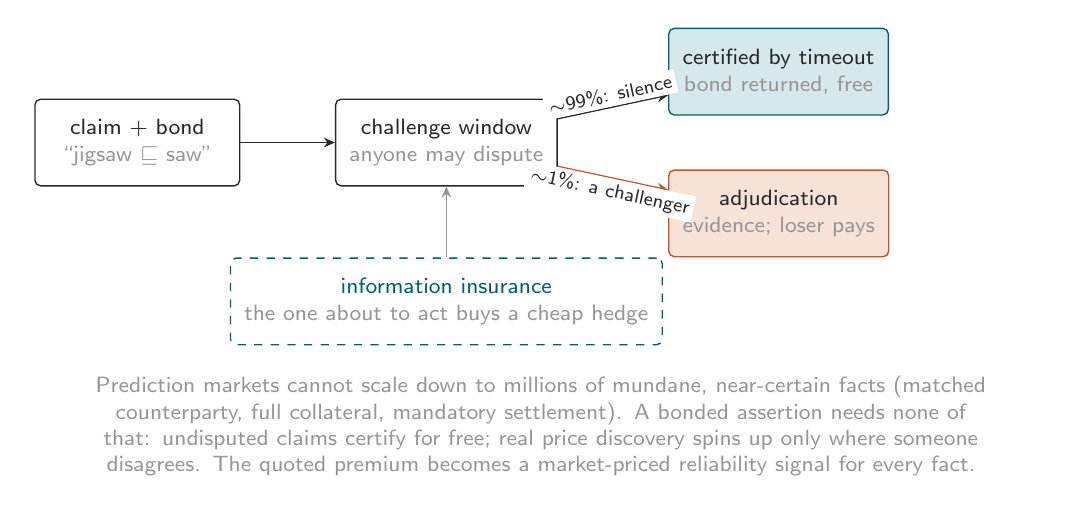
\begin{tikzpicture}[stg/.style={box, align=center, font=\footnotesize, minimum width=26mm, minimum height=11mm}]
  % The bonded-assertion lifecycle (optimistic-oracle shape): the bond is
  % sized to the cost of adjudication, not to the value at stake; the
  % expensive machinery runs only where someone disagrees.
  \node[stg] (assert) at (0,0) {claim + bond\\ {\color{soft}``jigsaw $\sqsubseteq$ saw''}};
  \node[stg, right=12mm of assert] (window) {challenge window\\ {\color{soft}anyone may dispute}};
  \node[stg, right=14mm of window, yshift=9mm, fill=accentlight, draw=accent] (cert) {certified by timeout\\ {\color{soft}bond returned, free}};
  \node[stg, right=14mm of window, yshift=-9mm, fill=warnlight, draw=warn] (adj) {adjudication\\ {\color{soft}evidence; loser pays}};
  \draw[flow] (assert) -- (window);
  \draw[flow] (window) -- node[lbl, sloped, above, font=\scriptsize] {$\sim$99\%: silence} (cert);
  \draw[wrong] (window) -- node[lbl, sloped, below, font=\scriptsize] {$\sim$1\%: a challenger} (adj);
  \node[stg, dashed, draw=accent, text=accent, below=9mm of window] (ins) {information insurance\\ {\color{soft}the one about to act buys a cheap hedge}};
  \draw[sub] (ins) -- (window);
  \node[note, text width=128mm] at ($(window) + (12mm,-36mm)$) {Prediction markets cannot scale down to millions of mundane, near-certain facts (matched counterparty, full collateral, mandatory settlement). A bonded assertion needs none of that: undisputed claims certify for free; real price discovery spins up only where someone disagrees. The quoted premium becomes a market-priced reliability signal for every fact.};
\end{tikzpicture}
\end{document}
